\documentclass{article}
\pagenumbering{arabic}
\newcommand{\newCommandName}{text to insert}
% Pages and colors used for the cover page
\usepackage{tikz-page}
\usepackage{url}
\usepackage{lastpage}

% Used for the math and code
\usepackage{amsmath}
\usepackage{listings}
\usepackage{pythonhighlight} % Got this from github! https://github.com/olivierverdier/python-latex-highlighting/blob/master/pythonhighlight.sty

% Used for the pictures
\usepackage{float}
\usepackage{graphicx}

% For the table
\usepackage[utf8]{inputenc}
\usepackage{multirow}
\usepackage{colortbl}
\usepackage{array}
\usepackage{tabularray}
\usepackage{nicematrix}

\usepackage[
  top=2cm,
  bottom=2cm,
  left=3cm,
  right=2cm,
  headheight=17pt, % as per the warning by fancyhdr
  includehead,includefoot,
  heightrounded, % to avoid spurious underfull messages
]{geometry} 

% Page numbers/header
\usepackage{fancyhdr}
\definecolor{brickred}{rgb}{0.8, 0.25, 0.33}
\definecolor{cobalt}{rgb}{0.0, 0.28, 0.67}
\definecolor{cadetgrey}{rgb}{0.57, 0.64, 0.69}

% Defining the text box being used for DEPT OF ENG
\tikzset{
        secnode/.style={
                minimum height = .16in,
                minimum width = 4.16in,
                inner xsep = 2pt,
                anchor=north east,
                draw=cadetgrey,
                fill=white,
                text=brickred,
                },
        }


         
\pagestyle{plain}
\renewcommand{\headrulewidth}{0pt}
\begin{document}


% Put name data and assignment number here
\newcommand\personaldate{April 14, 2024}
\newcommand\myname{Leo Berman}
\newcommand\myemail{leo.berman@temple.edu}
\newcommand\hwnum{08}
\newcommand\mynameabbrev{L. Berman}
\newcommand\assignmenttitle{LDA, K-NEAREST NEIGHBORS AND K-MEANS CLUSTERING}
\newcommand\yourclass{ECE 8527: Machine Learning and Pattern Recognition}
\begin{titlepage}
	% Drawing the border and the text box 
	\newcommand{\tikzpagelayout}{
		\draw[line width = .04in,
			color = cobalt]
		($(current page.north west)+(1in,-1in)$)
		rectangle ($(current page.south east)+(-.625in,1in)$);

		\draw[line width = .04in,
			color = brickred]
		($(current page.north west)+(.92in,-.92in)$)
		rectangle ($(current page.south east)+(-.705in,1.08in)$);
		\node[secnode] at ($(current page.north west)+(6in,-.875in)$) {\small{\textbf{DEPARTMENT OF ELECTRICAL AND COMPUTER ENGINEERING}}};
	}

	\begin{center}
		\large{Homework Assignment No. \hwnum:}\break
		\break
		\large{\textbf{HW No. \hwnum: \assignmenttitle}}\break
		\break
		\large{submitted to \:}\break
		\break
		\large{Professor Joseph Picone}\break
		\large{ECE 8527: Introduction to Pattern Recognition and Machine Learning}\break
		\large{Temple University}\break
		\large{College of Engineering}\break
		\large{1947 North 12th Street}\break
		\large{Philadelphia, Pennsylvania 19122}\break
		\break
		\large{\personaldate}\break
		\break
		\large{prepared by: }\break
		\break
		\large{\myname}\break
		\large{Email: \myemail}
	\end{center}
\end{titlepage}

\newpage
\pagestyle{fancy}
\fancyhead{}
\fancyfoot{}
\fancyhead[R,EH]{Page \thepage\ of \pageref{LastPage}}
\fancyhead[L,EH]{\mynameabbrev: HW \# \hwnum}
\fancyfoot[L,EF]{\yourclass}
\fancyfoot[R,EF]{\personaldate}
\renewcommand{\thesection}{\Alph{section}.}

\section{\MakeUppercase{Data Table}}
\begin{center}
  \begin{tblr}{
  colspec = {X[c]X[c]X[c]X[c]X[c]},
  stretch = 0,
  rowsep = 6pt,
  hlines = {black, 1pt},
  vlines = {black, 1pt},
  column{1} = {.5cm},
  column{2-6} = {2.25cm},
    }
     DS & System & Training Data & Train & Dev & {Eval} \\
     \multirow{14}{*}{08} & KNN(PAPER) & \multirow{8}{*}{/train} & 76.52 & 73.38 & 35.82 \\
     &RNF(PAPER) & & 70.77 & 60.55 & 40.23 \\
     & CI-PCA & & 36.07 & 36.02 & 31.76 \\
     & QDA & & 49.92 & 49.78 & 46.34 \\
     & LDA & & 36.09 & 36.01 & 31.94 \\
     & KNN & & 75.19 & 74.14 & 35.92 \\
     & RNF & & 100.00 & 71.18 & 36.86 \\
     & KNM & & 35.47 & 35.42 & 33.22 \\
     & CI-PICA & \multirow{6}{*}{/train + /dev} & 36.08 & 36.01 & 31.76\\
     & QDA & & 49.93 & 49.78 & 46.34\\
     & LDA & & 36.09 & 36.02 & 31.96\\
     & KNN & & 83.81 & 84.26 & 38.10\\
     & RNF & & 100.00& 100.00& 36.76\\
     & KNM & & 33.98 & 33.94 & 36.67 \\

     \multirow{14}{*}{09} & KNN(PAPER) & \multirow{8}{*}{/train} & 97.89 & 96.19 & 83.37 \\
     &RNF(PAPER) & & 97.94 & 96.18 & 81.68 \\
     & CI-PCA & & 96.20 & 91.82 & 97.36 \\
     & QDA & & 96.87 & 93.04 & 97.13 \\
     & LDA & & 96.20 & 91.82 & 97.36 \\
     & KNN & & 98.13 & 96.31 & 83.24 \\
     & RNF & & 100.00& 95.92 & 81.90 \\
     & KNM & & 87.13 & 84.69 & 90.96 \\
     & CI-PICA & \multirow{6}{*}{/train + /dev} & 95.93 & 91.80 & 97.11\\
     & QDA & & 97.15 & 93.84 & 96.68 \\
     & LDA & & 95.93 & 91.80 & 97.11\\
     & KNN & & 97.86 & 98.62 & 83.60\\
     & RNF & & 100.00& 100.00 & 80.89\\
     & KNM & & 84.47& 84.12 & 89.51\\
     
    \end{tblr}
\end{center}
\begin{figure}[H]
\begin{center}
  \begin{tblr}{
  colspec = {X[c]X[c]X[c]X[c]X[c]},
  stretch = 0,
  rowsep = 6pt,
  hlines = {black, 1pt},
  vlines = {black, 1pt},
  column{1} = {.5cm},
  column{2-6} = {2.25cm},
    }
     DS & System & Training Data & Train & Dev & {Eval} \\
     \multirow{14}{*}{10} & KNN(PAPER) & \multirow{8}{*}{/train} & 92.37 & 61.17 & 66.56 \\
     &RNF(PAPER) & & 97.85 & 20.27 & 66.72 \\
     & CI-PCA & & 53.02 & 51.13 & 48.90\\
     & QDA & & 83.92 & 55.24 & 65.89\\
     & LDA & & 53.02 & 50.13 & 48.90\\
     & KNN & & 92.48 & 61.37 & 66.53\\
     & RNF & & 100.00& 60.21 & 66.68\\
     & KNM & & 50.00 & 50.00 & 50.00\\
     & CI-PICA & \multirow{6}{*}{/train + /dev} & 53.03 & 50.75 & 48.99\\
     & QDA & & 85.00 & 56.90 & 65.30\\
     & LDA & & 53.03 & 50.75 & 48.99\\
     & KNN & & 94.29 & 89.64 & 62.89\\
     & RNF & & 100.00& 99.31 & 64.34\\
     & KNM & & 53.30 & 51.34 & 48.86\\     
    \end{tblr}
\end{center}
\caption{Data Table}
\end{figure}
\pagebreak
\section{\MakeUppercase{Plotting The Original Data}}
\begin{figure}[H]
	\centering
	\begin{minipage}{.33\textwidth}
			\centering
			\includegraphics[width=1\linewidth]{../Trainset 08.png}
			\caption{Training Set 8}
	\end{minipage}\hfill
        \centering
	\begin{minipage}{.33\textwidth}
			\centering
			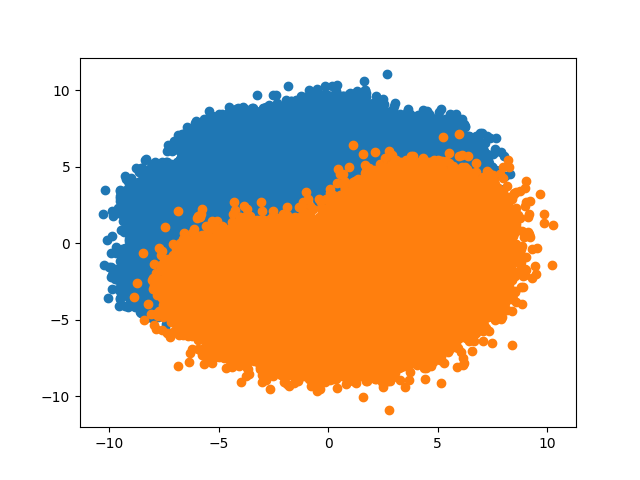
\includegraphics[width=1\linewidth]{../TrainSet 09.png}
			\caption{Training Set 9}
	\end{minipage}\hfill
        \centering
	\begin{minipage}{.33\textwidth}
			\centering
			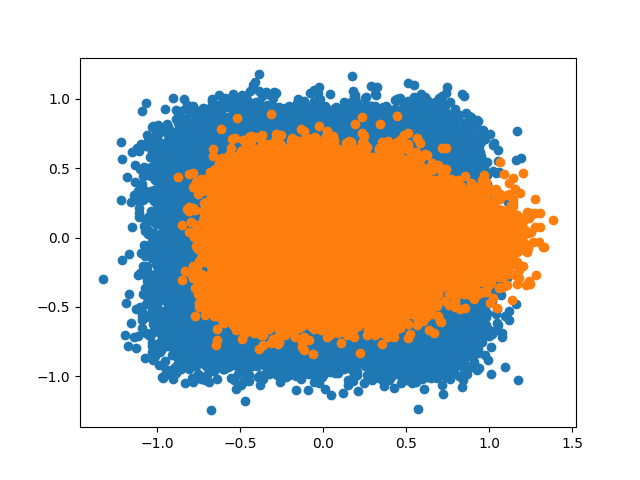
\includegraphics[width=1\linewidth]{../TrainSet 10.png}
			\caption{Training Set 10}
	\end{minipage}\hfill
\end{figure}
\begin{figure}[H]
	\centering
	\begin{minipage}{.33\textwidth}
			\centering
			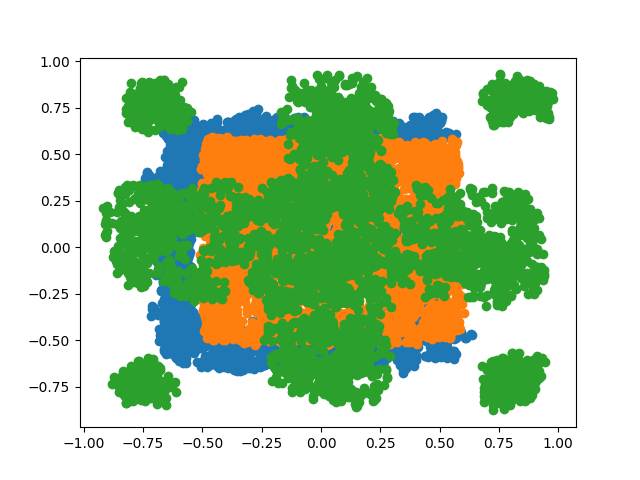
\includegraphics[width=1\linewidth]{../DevSet 08.png}
			\caption{Development Set 8}
	\end{minipage}\hfill
        \centering
	\begin{minipage}{.33\textwidth}
			\centering
			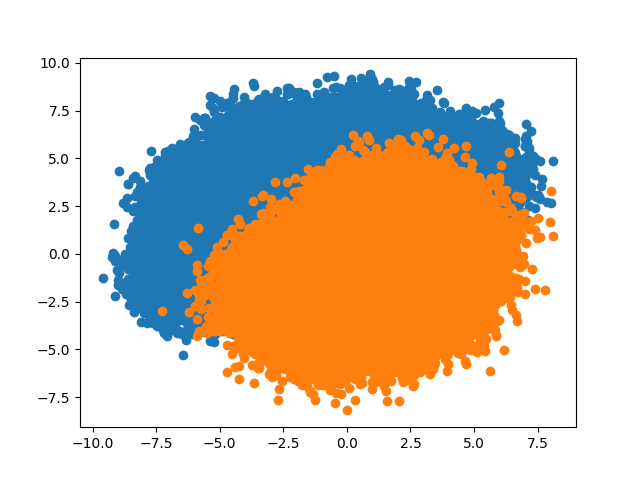
\includegraphics[width=1\linewidth]{../DevSet 09.png}
			\caption{Development Set 9}
	\end{minipage}\hfill
        \centering
	\begin{minipage}{.33\textwidth}
			\centering
			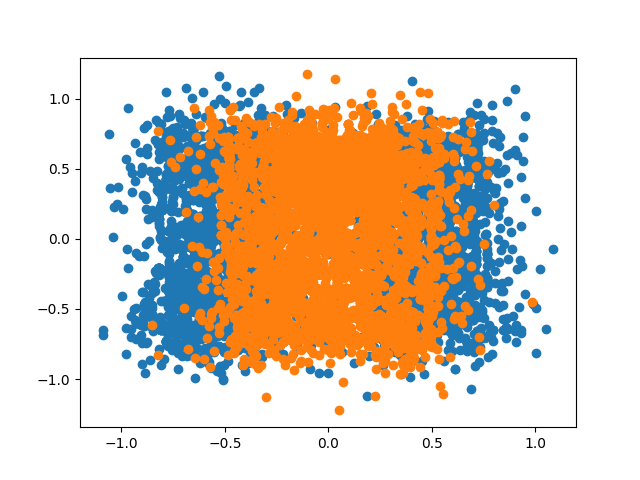
\includegraphics[width=1\linewidth]{../DevSet 10.png}
			\caption{Development Set 10}
	\end{minipage}\hfill
\end{figure}
\begin{figure}[H]
	\centering
	\begin{minipage}{.33\textwidth}
			\centering
			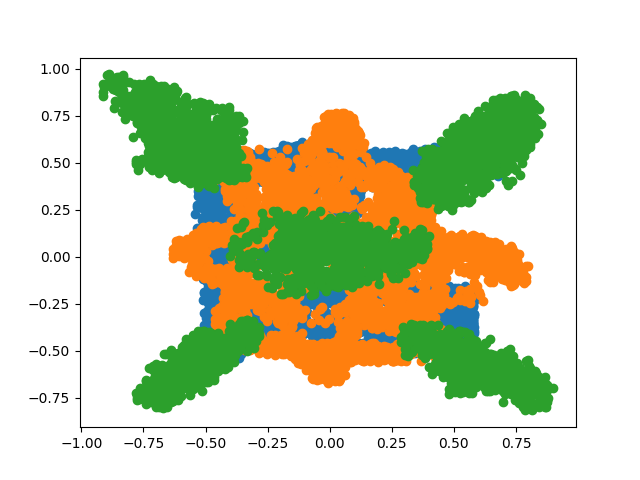
\includegraphics[width=1\linewidth]{../EvalSet 08.png}
			\caption{Evaluation Set 8}
	\end{minipage}\hfill
        \centering
	\begin{minipage}{.33\textwidth}
			\centering
			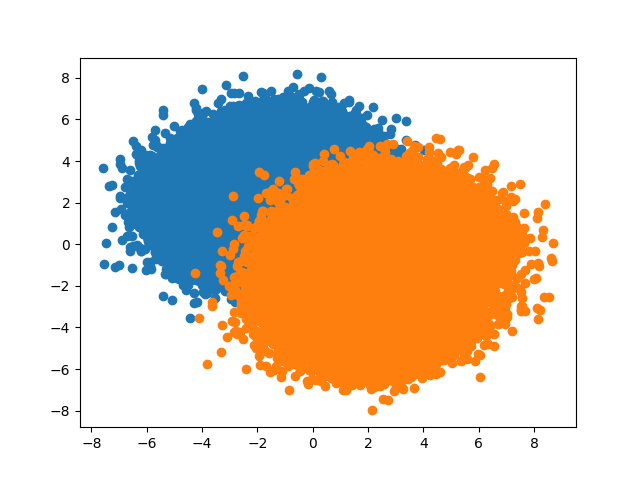
\includegraphics[width=1\linewidth]{../EvalSet 09.png}
			\caption{Evaluation Set 9}
	\end{minipage}\hfill
        \centering
	\begin{minipage}{.33\textwidth}
			\centering
			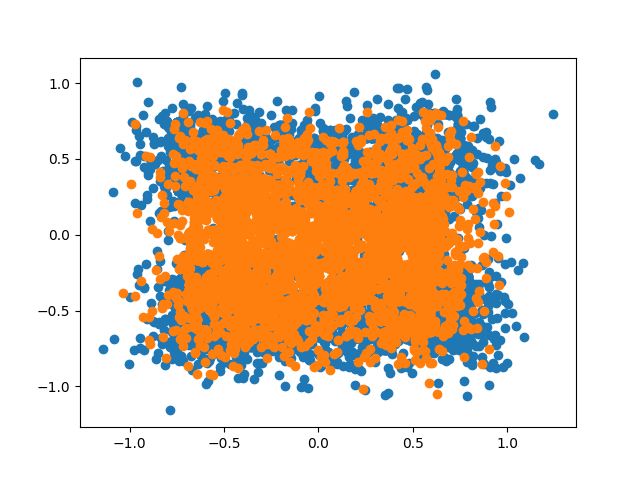
\includegraphics[width=1\linewidth]{../EvalSet 10.png}
			\caption{Evaluation Set 10}
	\end{minipage}\hfill
\end{figure}

\section{\MakeUppercase{Decision Surfaces}}
\begin{figure}[H]
	\centering
	\begin{minipage}{.33\textwidth}
			\centering
			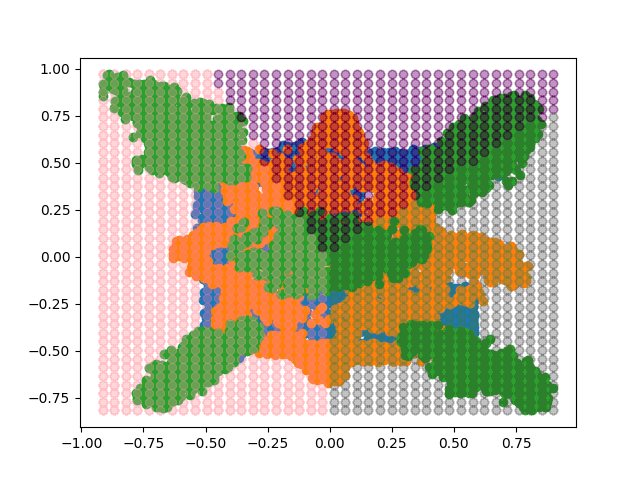
\includegraphics[width=1\linewidth]{../set8PCAdecisions.png}
			\caption{Set 8 PCA}
	\end{minipage}\hfill
        \centering
	\begin{minipage}{.33\textwidth}
			\centering
			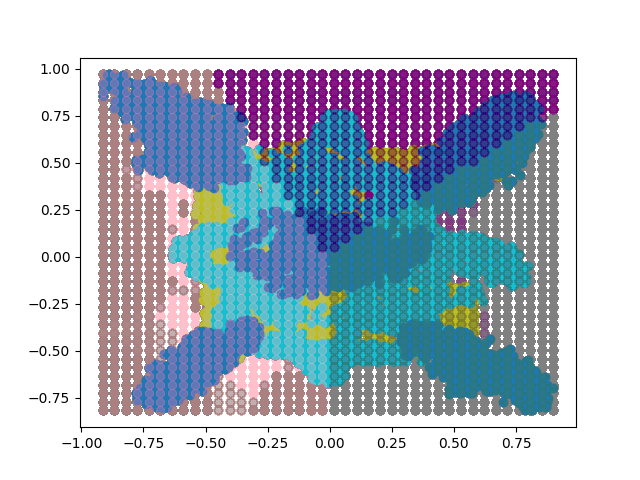
\includegraphics[width=1\linewidth]{../set9PCAdecisions.png}
			\caption{Set 9 PCA}
	\end{minipage}\hfill
        \centering
	\begin{minipage}{.33\textwidth}
			\centering
			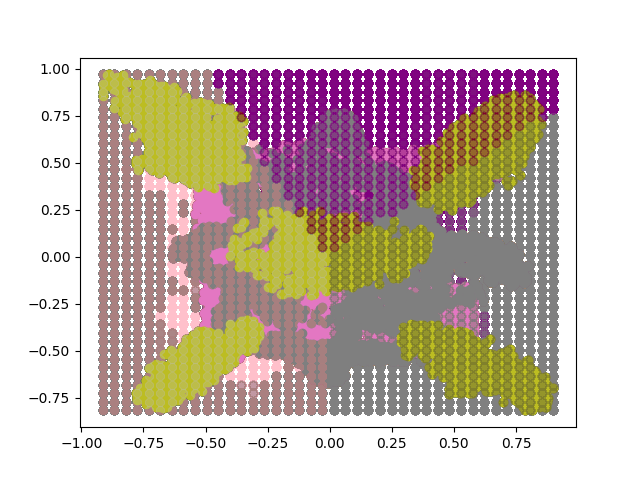
\includegraphics[width=1\linewidth]{../set10PCAdecisions.png}
			\caption{Set 10 PCA}
	\end{minipage}\hfill
\end{figure}

\begin{figure}[H]
	\centering
	\begin{minipage}{.33\textwidth}
			\centering
			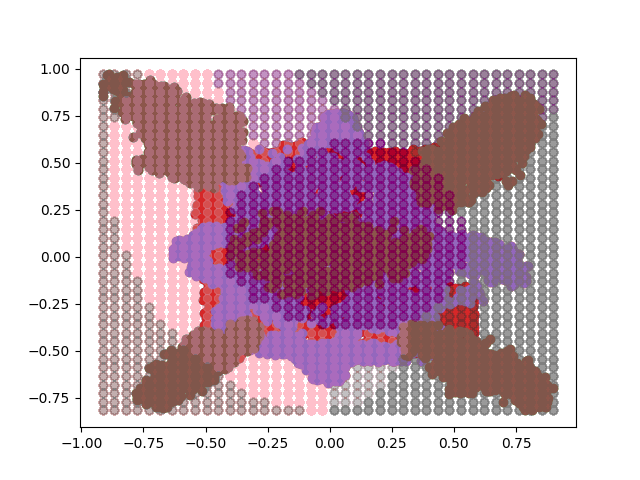
\includegraphics[width=1\linewidth]{../set8QDAdecisions.png}
			\caption{Set 8 QDA}
	\end{minipage}\hfill
        \centering
	\begin{minipage}{.33\textwidth}
			\centering
			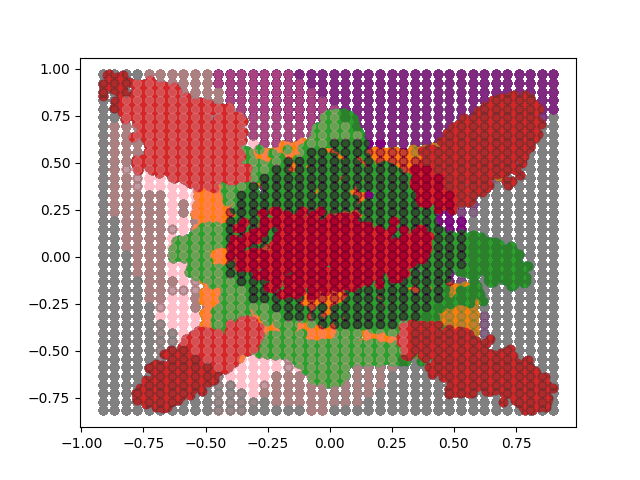
\includegraphics[width=1\linewidth]{../set9QDAdecisions.png}
			\caption{Set 9 QDA}
	\end{minipage}\hfill
        \centering
	\begin{minipage}{.33\textwidth}
			\centering
			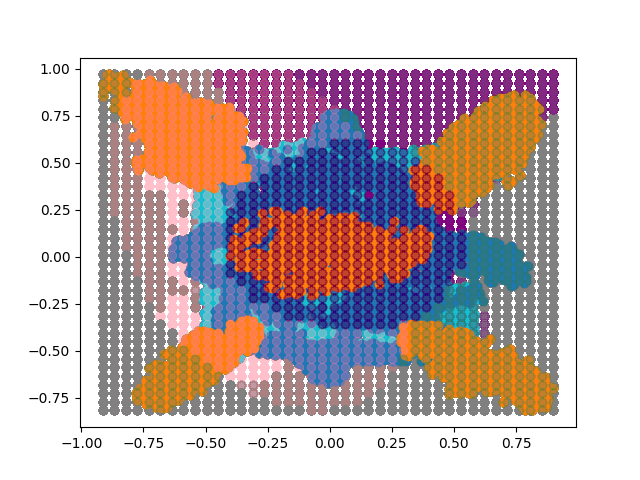
\includegraphics[width=1\linewidth]{../set10QDAdecisions.png}
			\caption{Set 10 QDA}
	\end{minipage}\hfill
\end{figure}

\begin{figure}[H]
	\centering
	\begin{minipage}{.33\textwidth}
			\centering
			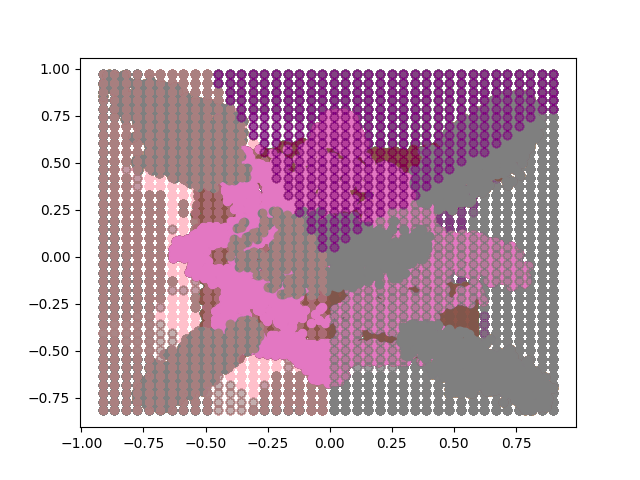
\includegraphics[width=1\linewidth]{../set8LDAdecisions.png}
			\caption{Set 8 LDA}
	\end{minipage}\hfill
        \centering
	\begin{minipage}{.33\textwidth}
			\centering
			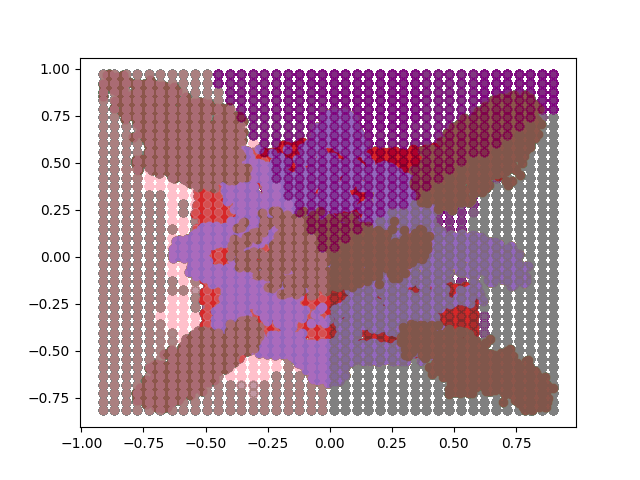
\includegraphics[width=1\linewidth]{../set9LDAdecisions.png}
			\caption{Set 9 LDA}
	\end{minipage}\hfill
        \centering
	\begin{minipage}{.33\textwidth}
			\centering
			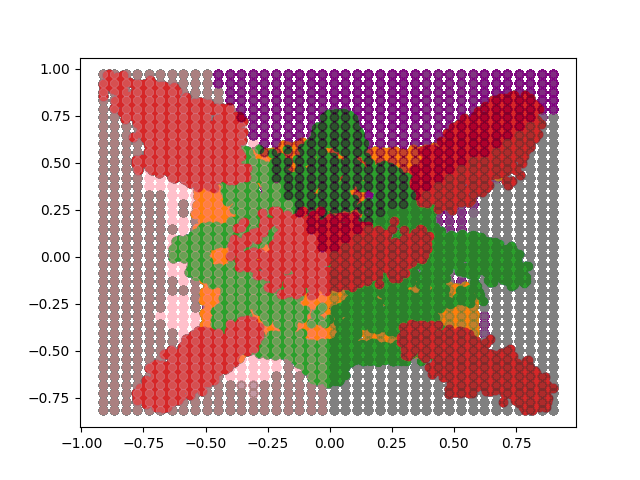
\includegraphics[width=1\linewidth]{../set10LDAdecisions.png}
			\caption{Set 10 LDA}
	\end{minipage}\hfill
\end{figure}

\begin{figure}[H]
	\centering
	\begin{minipage}{.33\textwidth}
			\centering
			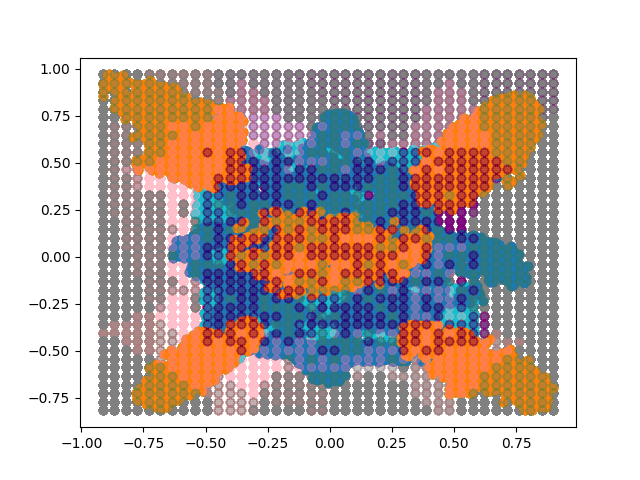
\includegraphics[width=1\linewidth]{../set8KNNdecisions.png}
			\caption{Set 8 KNN}
	\end{minipage}\hfill
        \centering
	\begin{minipage}{.33\textwidth}
			\centering
			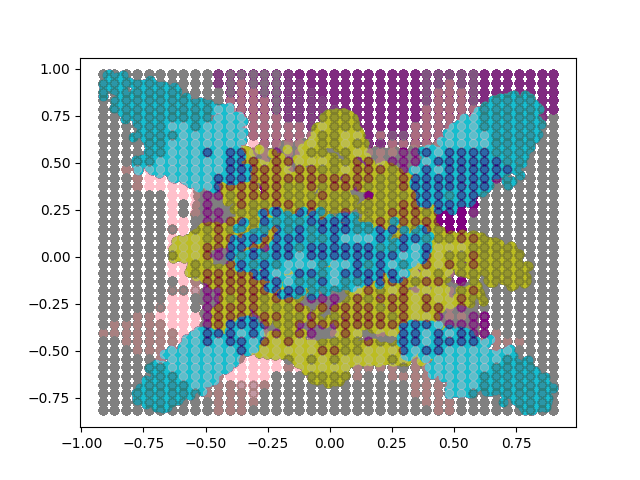
\includegraphics[width=1\linewidth]{../set9KNNdecisions.png}
			\caption{Set 9 KNN}
	\end{minipage}\hfill
        \centering
	\begin{minipage}{.33\textwidth}
			\centering
			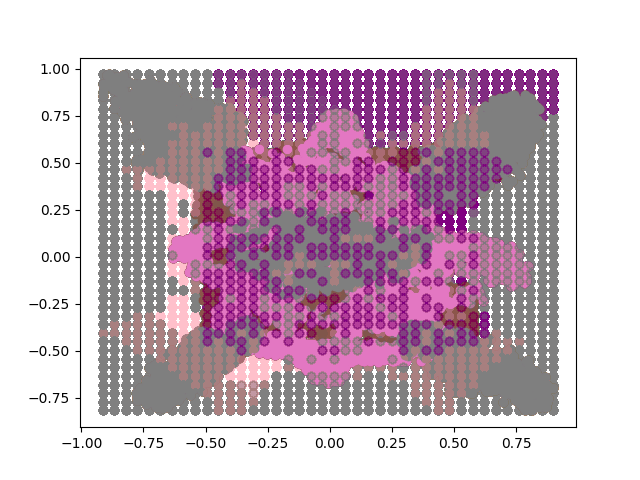
\includegraphics[width=1\linewidth]{../set10KNNdecisions.png}
			\caption{Set 10 KNN}
	\end{minipage}\hfill
\end{figure}

\begin{figure}[H]
	\centering
	\begin{minipage}{.33\textwidth}
			\centering
			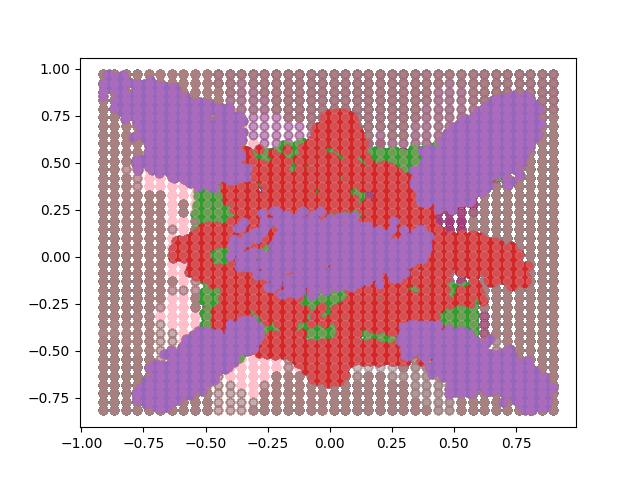
\includegraphics[width=1\linewidth]{../set8KNMdecisions.png}
			\caption{Set 8 KNM}
	\end{minipage}\hfill
        \centering
	\begin{minipage}{.33\textwidth}
			\centering
			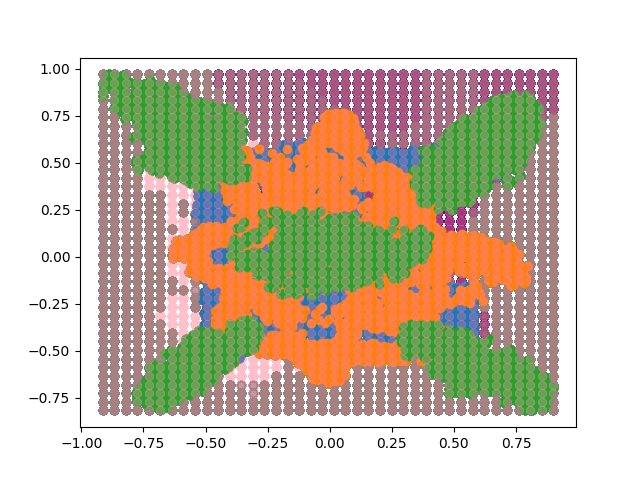
\includegraphics[width=1\linewidth]{../set9KNMdecisions.png}
			\caption{Set 9 KNM}
	\end{minipage}\hfill
        \centering
	\begin{minipage}{.33\textwidth}
			\centering
			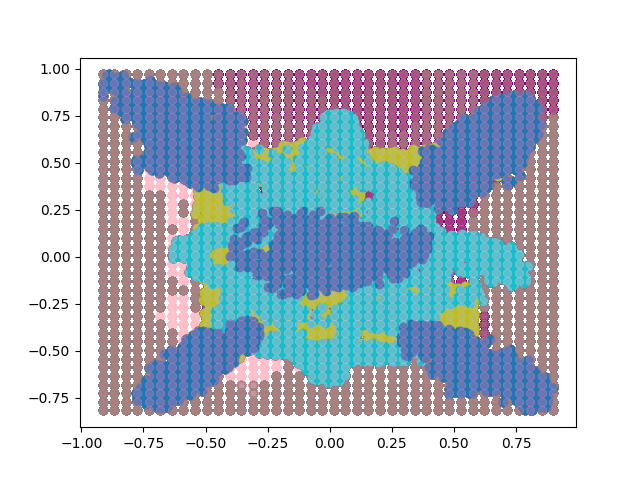
\includegraphics[width=1\linewidth]{../set10KNMdecisions.png}
			\caption{Set 10 KNM}
	\end{minipage}\hfill
\end{figure}




\section{\MakeUppercase{KNN and KNM Plots}}
\begin{figure}[H]
	\centering
	\begin{minipage}{.33\textwidth}
			\centering
			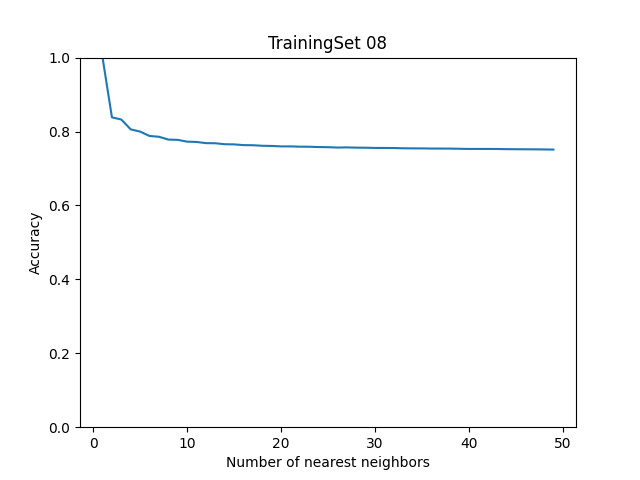
\includegraphics[width=1\linewidth]{../KNN_TrainingSet 08.png}
			\caption{Training Set 8}
	\end{minipage}\hfill
        \centering
	\begin{minipage}{.33\textwidth}
			\centering
			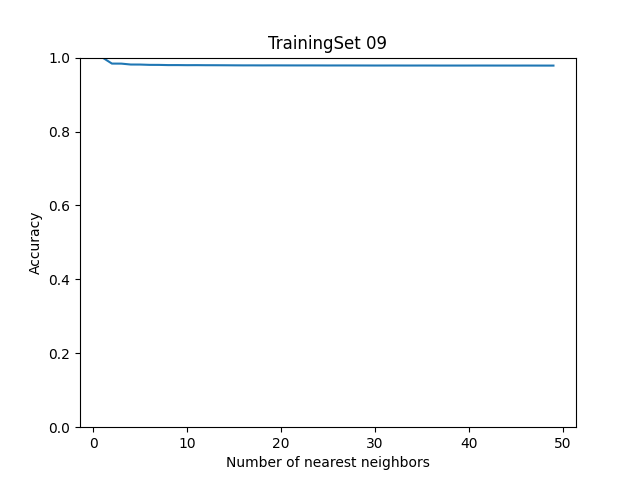
\includegraphics[width=1\linewidth]{../KNN_TrainingSet 09.png}
			\caption{Training Set 9}
	\end{minipage}\hfill
        \centering
	\begin{minipage}{.33\textwidth}
			\centering
			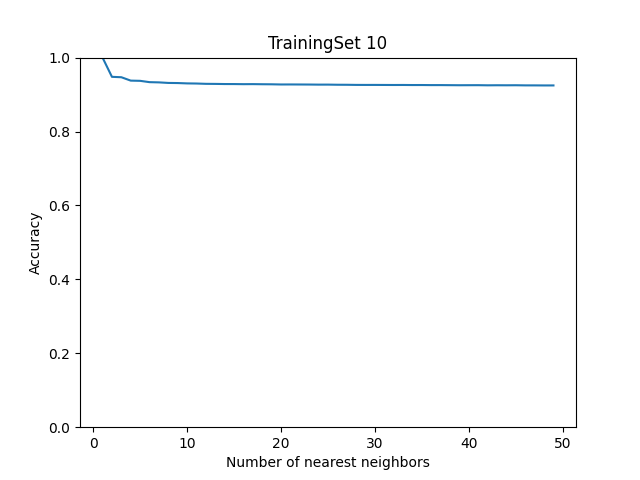
\includegraphics[width=1\linewidth]{../KNN_TrainingSet 10.png}
			\caption{Training Set 10}
	\end{minipage}\hfill
\end{figure}

\begin{figure}[H]
	\centering
	\begin{minipage}{.33\textwidth}
			\centering
			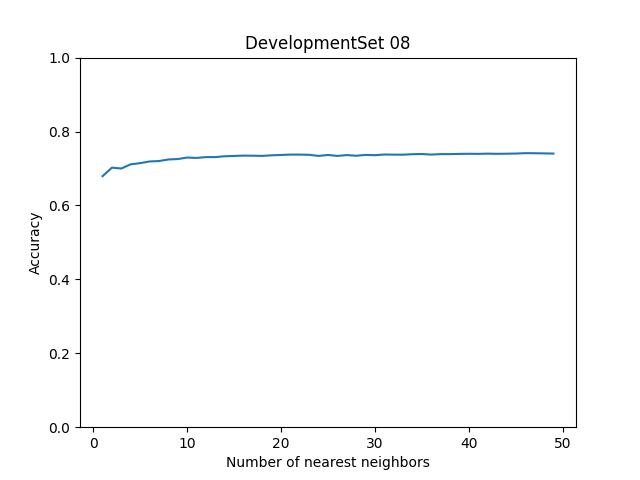
\includegraphics[width=1\linewidth]{../KNN_DevelopmentSet 08.png}
			\caption{Development Set 8}
	\end{minipage}\hfill
        \centering
	\begin{minipage}{.33\textwidth}
			\centering
			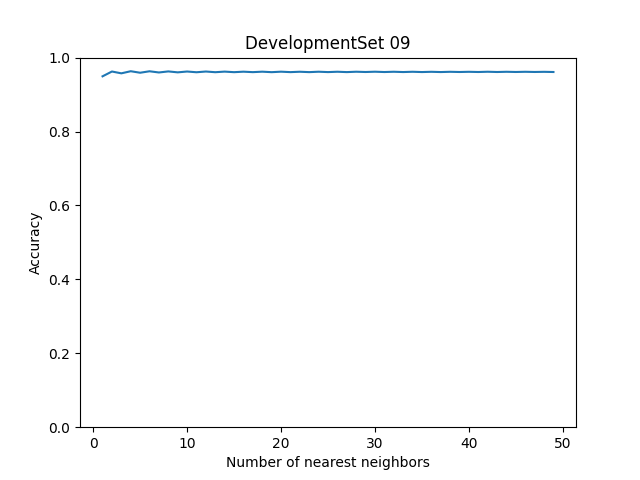
\includegraphics[width=1\linewidth]{../KNN_DevelopmentSet 09.png}
			\caption{Development Set 9}
	\end{minipage}\hfill
        \centering
	\begin{minipage}{.33\textwidth}
			\centering
			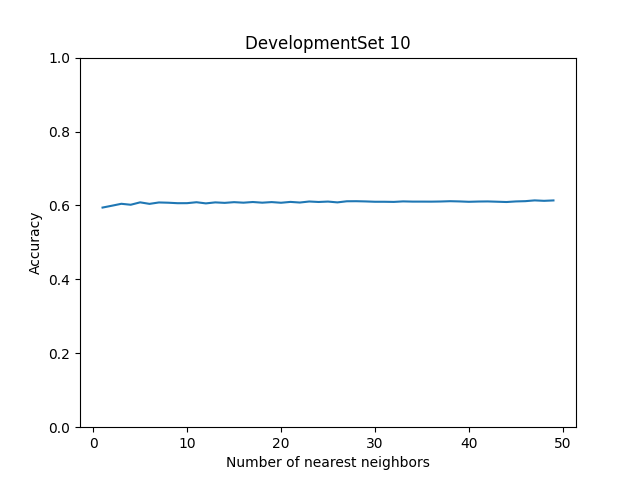
\includegraphics[width=1\linewidth]{../KNN_DevelopmentSet 10.png}
			\caption{Development Set 10}
	\end{minipage}\hfill
\end{figure}

\begin{figure}[H]
	\centering
	\begin{minipage}{.33\textwidth}
			\centering
			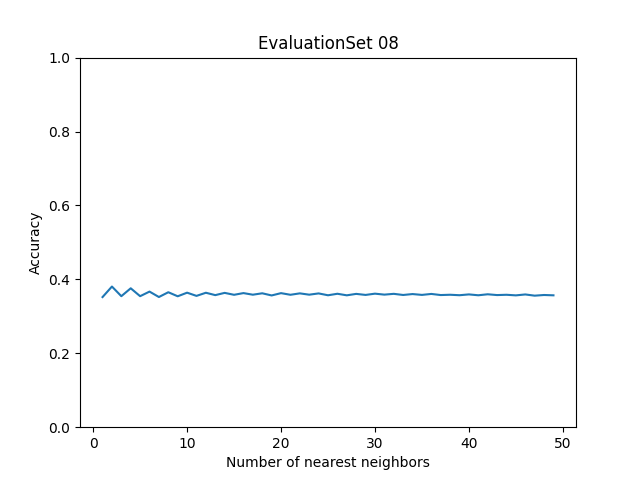
\includegraphics[width=1\linewidth]{../KNN_EvaluationSet 08.png}
			\caption{Evaluation Set 8}
	\end{minipage}\hfill
        \centering
	\begin{minipage}{.33\textwidth}
			\centering
			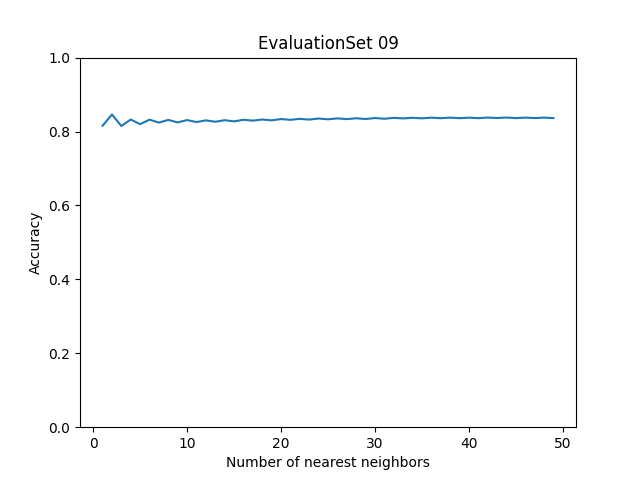
\includegraphics[width=1\linewidth]{../KNN_EvaluationSet 09.png}
			\caption{Evaluation Set 9}
	\end{minipage}\hfill
        \centering
	\begin{minipage}{.33\textwidth}
			\centering
			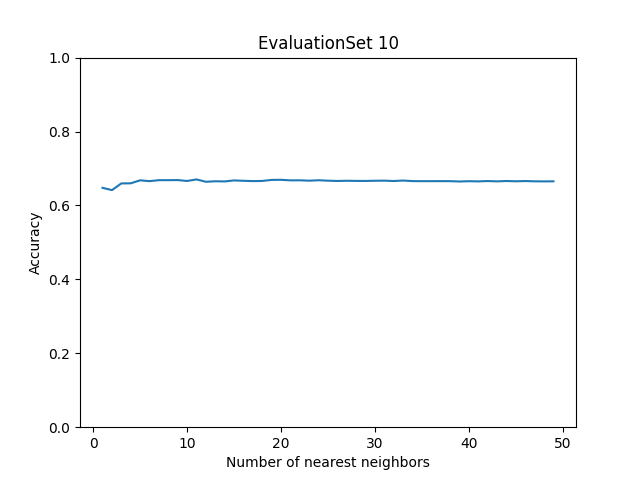
\includegraphics[width=1\linewidth]{../KNN_EvaluationSet 10.png}
			\caption{Evaluation Set 10}
	\end{minipage}\hfill
\end{figure}

\section{\MakeUppercase{Summary}}
\begin{flushleft}For dataset 8, we can see that our best result for the eval data was QDA. By calculating the mean and covariance for each dataset, we can see that even though it didn't do as well on the training and dev set, it generalized the data so although it wasn't able to separate the classes well and squash everything into matrixes well, it was consistent which is important.\break\break
For dataset 9, we can see that QDA, PCA, and LDA did really well which could hint that the classes are separated clearly on a dimensionally reduced plane. KNN, RNF, and KNM didn't do as well which could possibly be indicative of the lack of normalization being a problem.\break\break
For dataset 10, we can see that KNN, RNF, and QDA perform the best. This is indicative of their being a large amount of variance. Since LDA didn't do as well as QDA we can see that the variance of data might be higher which shows that QDA might be better.\break\break
In summary, we can see that overall QDA performs the best.

\end{flushleft}
\end{document}
